% --------------------------------------------------------------------------- %
% A0 paper poster for MetrumRG						   %
% --------------------------------------------------------------------------- %
% Created with Brian Amberg's LaTeX Poster Template. 					     %
% --------------------------------------------------------------------------- %

\documentclass[a0paper,portrait]{baposter}

\usepackage{relsize}		% For \smaller
\usepackage{url}			% For \url
\usepackage{epstopdf}	% Included EPS files automatically converted to PDF to include with pdflatex
\usepackage{graphicx}
\usepackage{setspace}
\spacing{1}
\usepackage{anyfontsize}


\usepackage[bitstream-charter]{mathdesign}
\usepackage[T1]{fontenc}

% Deprecating osfigures option; use oldstyle instead; 2020-09-10
\usepackage[defaultsans,oldstyle,scale=0.95]{opensans}

%%% Global Settings %%%%%%%%%%%%%%%%%%%%%%%%%%%%%%%%%%%%%%%%%%%%%%%%%%%%%%%%%%%

\graphicspath{{pix/}}	% Root directory of the pictures 
\tracingstats=2			% Enabled LaTeX logging with conditionals

%%% Color Definitions %%%%%%%%%%%%%%%%%%%%%%%%%%%%%%%%%%%%%%%%%%%%%%%%%%%%%%%%%

\definecolor{bordercol}{RGB}{40,40,40}
\definecolor{headercol1}{RGB}{186,215,230}
\definecolor{headercol2}{RGB}{80,80,80}
\definecolor{headerfontcol}{RGB}{0,0,0}
\definecolor{boxcolor}{RGB}{186,215,230}
\definecolor{metgreen}{rgb}{0,0.555,0}
\definecolor{lightergreen}{rgb}{.8,1,0.85}
\definecolor{lightergray}{RGB}{225,225,225}
\definecolor{darkteal}{RGB}{41, 127, 157}
\definecolor{tealdark}{RGB}{41, 104, 157}
\definecolor{black}{RGB}{0,0,0}

% PLEASE MODIFY COLOR SCHEME HERE IF NEEDED
\colorlet{titlefgcol}{black}
\colorlet{headerbgcol}{darkteal}
\colorlet{headerfgcol}{white}
\colorlet{bordercol}{lightergray}
\newcommand{\headershade}{none}

%%%%%%%%%%%%%%%%%%%%%%%%%%%%%%%%%%%%%%%%%%%%%%%%%%%%%%%%%%%%%%%%%%%%%%%%%%%%%%%%
%%% Utility functions %%%%%%%%%%%%%%%%%%%%%%%%%%%%%%%%%%%%%%%%%%%%%%%%%%%%%%%%%%

%%% Save space in lists. Use this after the opening of the list %%%%%%%%%%%%%%%%
\newcommand{\compresslist}{
	\setlength{\itemsep}{1pt}
	\setlength{\parskip}{0pt}
	\setlength{\parsep}{0pt}
}

%%%%%%%%%%%%%%%%%%%%%%%%%%%%%%%%%%%%%%%%%%%%%%%%%%%%%%%%%%%%%%%%%%%%%%%%%%%%%%%
%%% Document Start %%%%%%%%%%%%%%%%%%%%%%%%%%%%%%%%%%%%%%%%%%%%%%%%%%%%%%%%%%%%
%%%%%%%%%%%%%%%%%%%%%%%%%%%%%%%%%%%%%%%%%%%%%%%%%%%%%%%%%%%%%%%%%%%%%%%%%%%%%%%

\begin{document}
\typeout{Poster rendering started}

%%% Setting Background Image %%%%%%%%%%%%%%%%%%%%%%%%%%%%%%%%%%%%%%%%%%%%%%%%%%
\background{
%	\begin{tikzpicture}[remember picture,overlay]%
%	\draw (current page.north west)+(-2em,2em) node[anchor=north west]
%	{\includegraphics[height=1.1\textheight]{background}};
%	\end{tikzpicture}
}

%%% General Poster Settings %%%%%%%%%%%%%%%%%%%%%%%%%%%%%%%%%%%%%%%%%%%%%%%%%%%
%%%%%% Eye Catcher, Title, Authors and University Images %%%%%%%%%%%%%%%%%%%%%%
\begin{poster}{
	grid=false,
	% Option is left on true though the eyecatcher is not used. The reason is
	% that we have a bit nicer looking title and author formatting in the headercol
	% this way
	% columns = 4,
	eyecatcher=false, 
	borderColor=bordercol,
	headerColorOne=headerbgcol,
	headerColorTwo=headerbgcol,
	headerFontColor=headerfgcol,
	% Only simple background color used, no shading, so boxColorTwo isn't necessary
	boxColorOne=white,
	headershape=rectangle,
	headerfont=\Large\bf\textsf,
	textborder=rectangle,
	background=user,
	headerborder=open,
  boxshade=none, 
  headershade=plain,
  headerheight=0.1\textheight %% CHANGE THIS TO INCREASE ROOM FOR LONG TITLE
}
%%% Eye Cacther %%%%%%%%%%%%%%%%%%%%%%%%%%%%%%%%%%%%%%%%%%%%%%%%%%%%%%%%%%%%%%%
{
%	Eye Catcher, empty if option eyecatcher=false - unused
}
%%% Title %%%%%%%%%%%%%%%%%%%%%%%%%%%%%%%%%%%%%%%%%%%%%%%%%%%%%%%%%%%%%%%%%%%%%
{
	\textbf{\textsf{\color{titlefgcol}{
	\huge
	  A multi-organ integrated QSP model for hematopoietic stem cell differentiation to predict the immune cell reconstitution in ex-vivo gene therapy
	 }}}\vspace{.5em}
}
%%% Authors %%%%%%%%%%%%%%%%%%%%%%%%%%%%%%%%%%%%%%%%%%%%%%%%%%%%%%%%%%%%%%%%%%%
{
\normalsize
	Yuezhe Li$^1$, Eric Jordie$^1$, Tim Knab$^1$\\
	{\smaller
	  $^1$\textit{Metrum Research Group}
	}
}
%%% Logo %%%%%%%%%%%%%%%%%%%%%%%%%%%%%%%%%%%%%%%%%%%%%%%%%%%%%%%%%%%%%%%%%%%%%%
{
% The logos are compressed a bit into a simple box to make them smaller on the result
% (Wasn't able to find any bigger of them.)
%\setlength\fboxsep{5pt}
%\setlength\fboxrule{0.5pt}
%	\fbox{
		\begin{minipage}{16em}
			\begin{center}
			
\includegraphics[width=14em]{newlogo} 
			\end{center}
		\end{minipage}
%	}
}
%%%%%%%%%%%%%%%%%%%%%%%%%%%%%%%%%%%%%%%%%%%%%%%%%%%%%%%%%%%%%%%%%%%%%%%%%%%%%%%%
%%%%%%%%%%%%%%%%%%%%%%%%%%%%%%%%%%%%%%%%%%%%%%%%%%%%%%%%%%%%%%%%%%%%%%%%%%%%%%%%


\headerbox{Abstract}{name=abstract,column=0,row=0}{
\footnotesize

The differentiation of mammalian hematopoietic stem cells (HSCs) is complex and multi-scale, providing an opportunity for mathematical modeling and simulation to aid in mechanistic understanding and ultimately inform drug development efforts. Historically, mathematical models have been developed that were focused on the development of a subset of cells, but mathematical models that encompass the overall cellular system’s complexity are rarely available. Here, we develop an integrated quantitative systems pharmacology (QSP) model that characterizes multi-organ recapitulation of HSC differentiation by integrating literature models and adding novel features. The result is a more comprehensive representation of mammalian hematopoietic stem cell development. We demonstrate our integrated model can accurately capture the reconstitution of RBCs, B cells, and T cells following HSC transplant in mice. Moreover, the humanized model successfully predicted the reconstitution of granulocytes and lymphocytes  in patients with adenosine deaminase‐deficient severe combined immunodeficiency (ADA-SCID) who underwent ex-vivo gene therapy. 


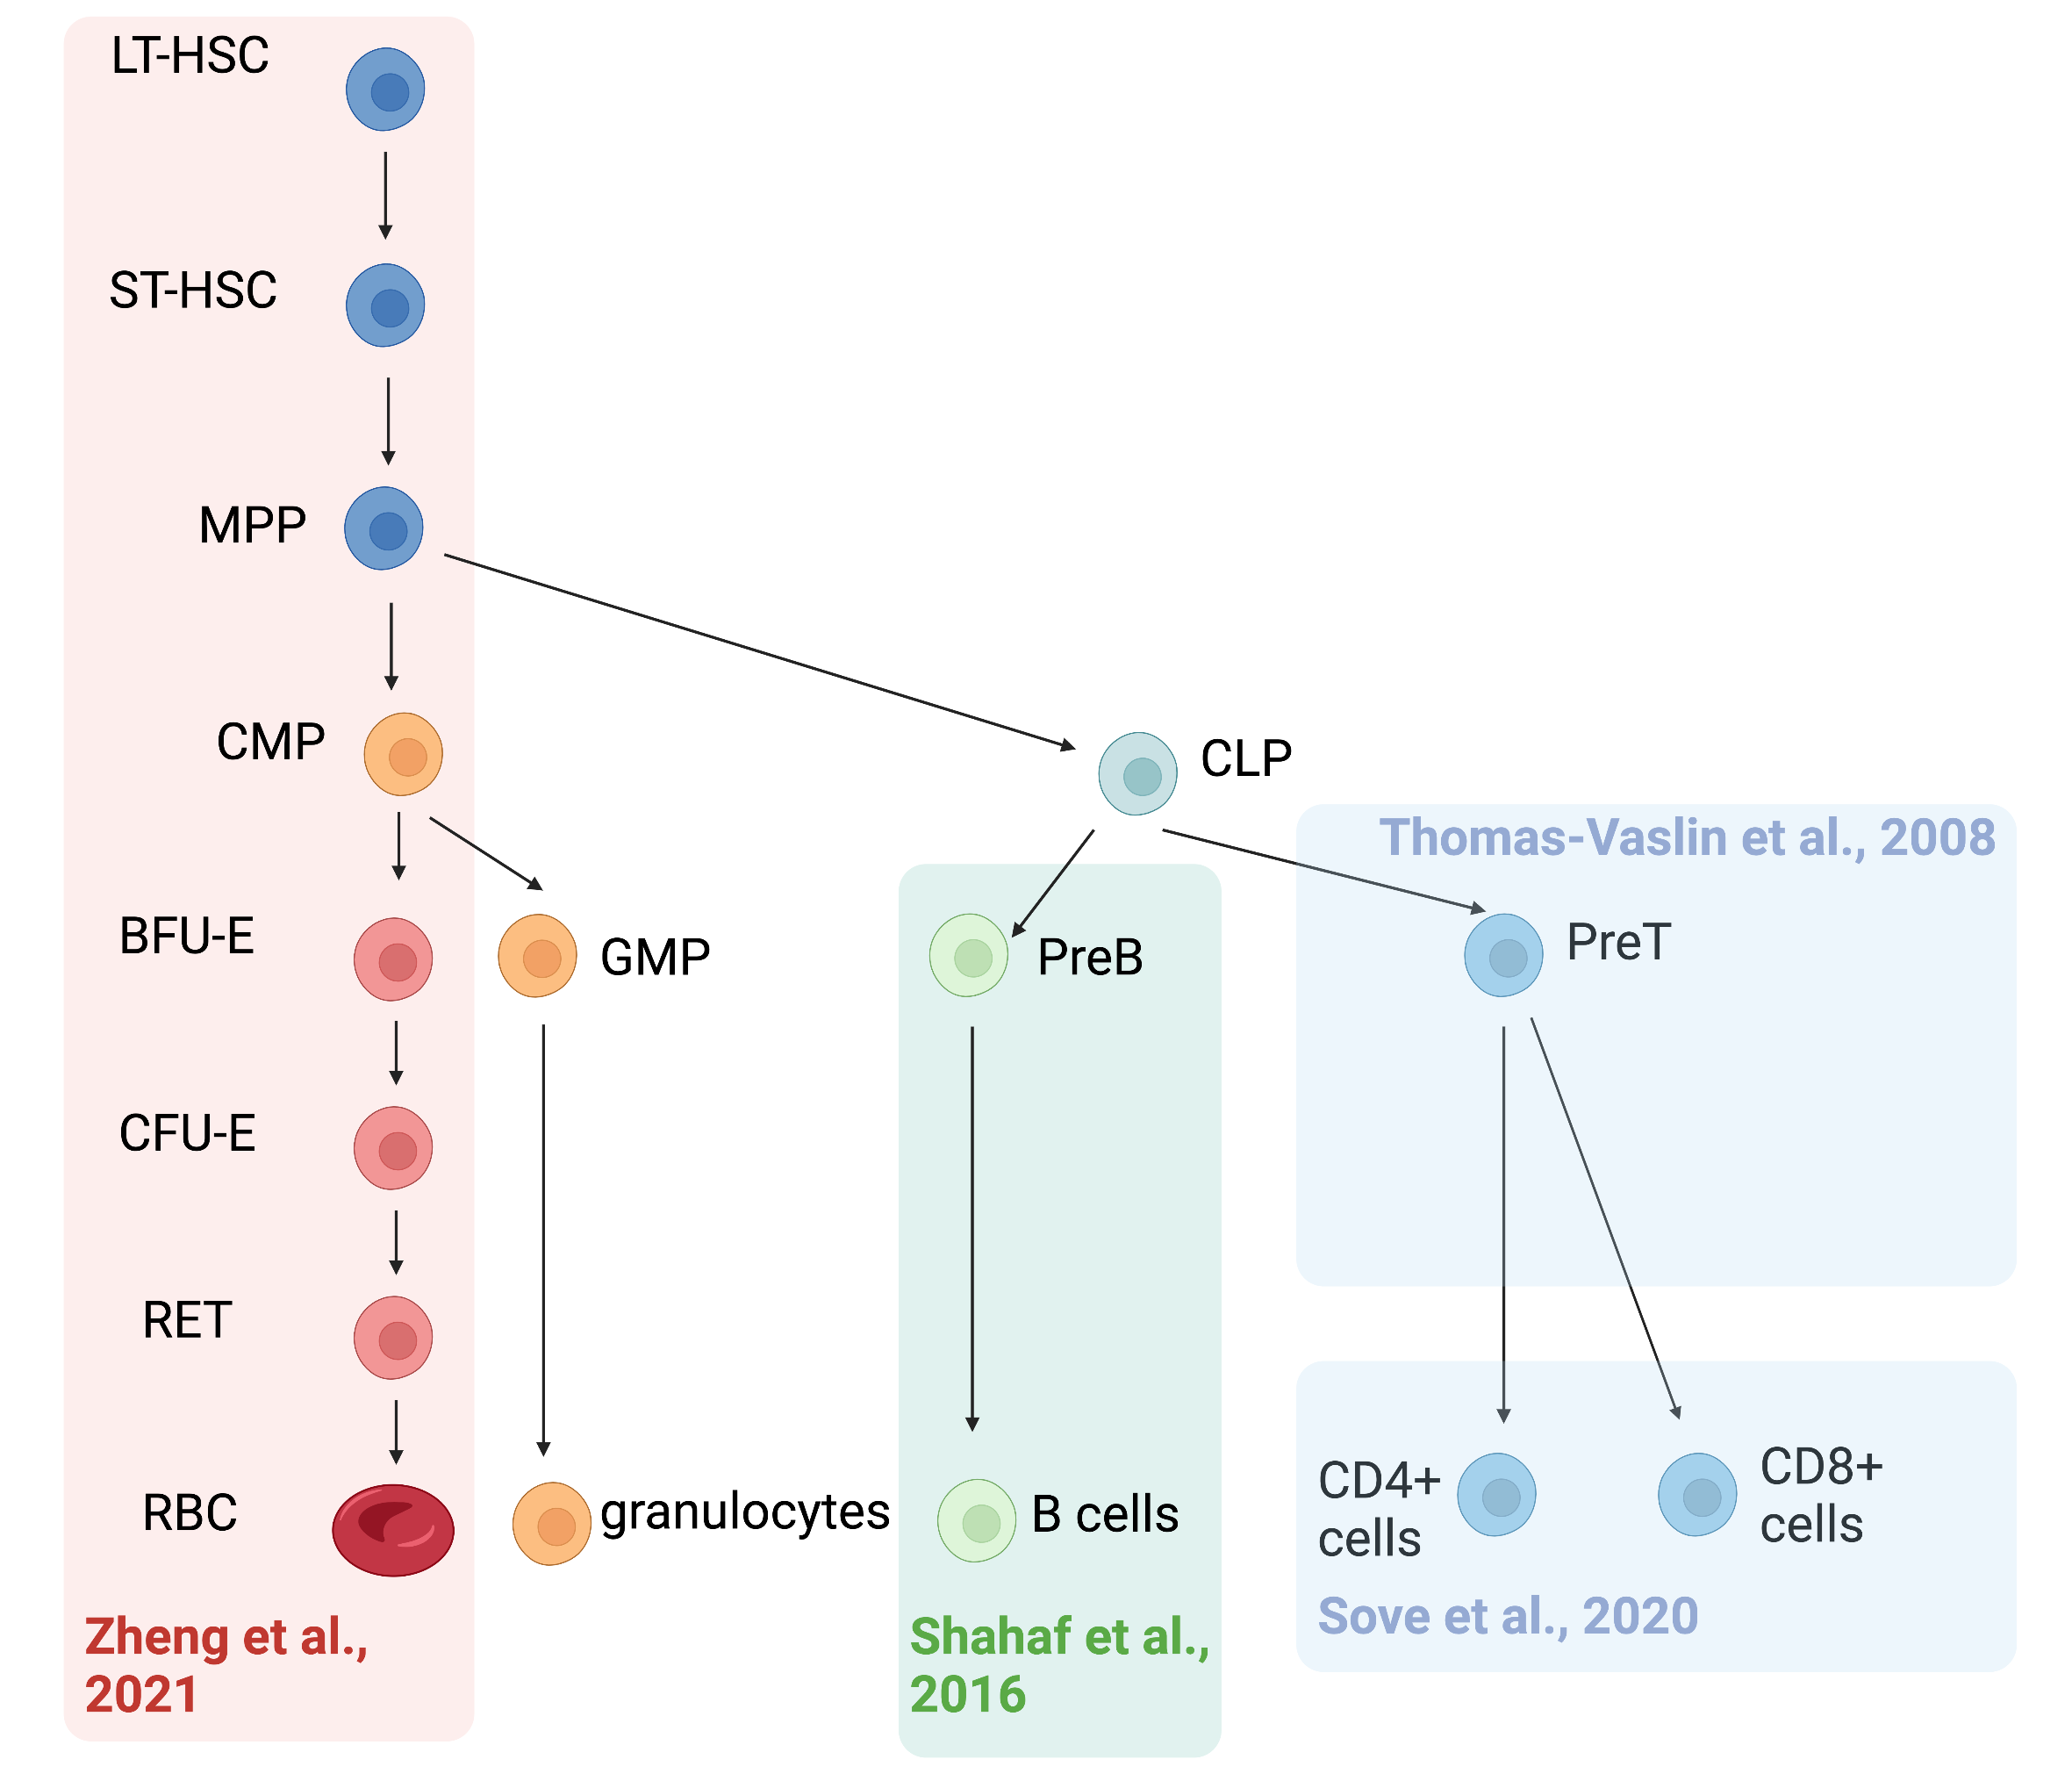
\includegraphics[width= 0.8 \textwidth]{../img/Diagram_integration}

}
%%%%%%%%%%%%%%%%%%%%%%%%%%%%%%%%%%%%%%%%%%%%%%%%%%%%%%%%%%%%%%%%%%%%%%%%%%%%%%%%

\headerbox{Methods}{name=methods,column=0,below=abstract}{
\footnotesize

We developed an integrated model that depicts the differentiation of hematopoietic stem cells (HSCs) into erythrocytes, lymphocytes, and granulocytes. The model was built incrementally by incorporating novel physiological-based features from literature while integrating published models:
\begin{itemize}
%\setlength{\itemindent}{-2em}
  \item human HSC differentiation into red blood cells (RBCs) [1]
  \item mouse B cell development [2]
  \item mouse T cell development [3]
  \item human naive T cell dynamics model [4]
\end{itemize}

The model was developed in 4 steps: 
\begin{itemize}
  \item Implement an existing human HSC -> RBC differentiation model in [1]
  \item Scale the HSC -> RBC differentiation model from human to mouse
  \item Integrate T cells development model from [3], B cells development model from [2], and HSC -> granulocyte differentiation model into the mouse differentiation model 
  \item Scale the integrated mouse HSC differentiation model to human.
\end{itemize}

Further parameter tunings were carried out using steady state data (e.g. cell ratios in blood or other organs) in mouse and in human. The integrated models for mouse and human were validated using cell reconstitution in peripheral blood after stem cell transplant/ ex-vivo gene therapy. 

}

%%%%%%%%%%%%%%%%%%%%%%%%%%%%%%%%%%%%%%%%%%%%%%%%%%%%%%%%%%%%%%%%%%%%%%%%%%%%%%%%

\headerbox{References}{name=references,column=0,below=methods}{
\scriptsize	
[1] Zheng, Bo, et al. "A systems pharmacology model for gene therapy in sickle cell disease." CPT: Pharmacometrics \& Systems Pharmacology 10.7 (2021): 696-708.
[2] Shahaf, Gitit, et al. "B cell development in the bone marrow is regulated by homeostatic feedback exerted by mature B cells." Frontiers in immunology 7 (2016): 77.
[3] Thomas-Vaslin, Veronique, et al. "Comprehensive assessment and mathematical modeling of T cell population dynamics and homeostasis." The Journal of Immunology 180.4 (2008): 2240-2250.
[4] Sové, Richard J., et al. "QSP‐IO: a quantitative systems pharmacology toolbox for mechanistic multiscale modeling for Immuno‐oncology applications." CPT: pharmacometrics \& systems pharmacology 9.9 (2020): 484-497.


}


\headerbox{Source code}{name=code,column=0,below=references}{

\includegraphics[width= 0.1\textwidth]{../img/repo_qr_code.png}
}


%%%%%%%%%%%%%%%%%%%%%%%%%%%%%%%%%%%%%%%%%%%%%%%%%%%%%%%%%%%%%%%%%%%%%%%%%%%%%%%%
%%%%%%%%%%%%%%%%%%%%%%%%%%%%%%%%%%%%%%%%%%%%%%%%%%%%%%%%%%%%%%%%%%%%%%%%%%%%%%%%


\headerbox{Results}{name=results,span=2,column=1,row=0}{
\footnotesize

The integrated HSC differentiation model for mouse can be summarized by the figure follow. 
Briefly, the long-term hematopoietic stem cells (LT-HSC) is capable of self-renewal and can differentiate to be short-term hematopoietic stem cells (ST-HSC). 
ST-HSC can differentiate to be multipottrnt ptogrnitor cells (MPP). 
MPP can differentiate to be common myeloid progenitor (CMP) or common lymphoid progenitor (CLP). 
CMP can differentitiate to be burst forming unit-erythroid (BFU-E) and granulocyte-monocyte progenitors (GMP). 
BFU-E can differentiate to be colony forming unit-erythroid (CFU-E), then reticulocytes (RET) and red blood cells (RBC). Furthermore, hemoglobin (Hb) can be synthesized in RETs and RBCs, and the oxygen level in blood imposes a negative feedback on CFU-E amplification. 
The erythrocytes differentiation model was taken from [1]  and scaled from human to mouse by reparameterize of mean residence time and amplification number is based on rates and observations provided in Busch et al., Nature. 2015, Putten and Croon, Blood. 1958, Ney Curr Opin Hematol. 2011, and Palis, Front Physio. 2014.  
CLP can further differentiate into B cells and T cells in bone marrow, spleen (diagram in middle panel, model obtained from [2]) and thymus (diagram in right panel, model obtained from [3]). 
GMP can further differentiate to be granulocytes (GM). 


\begin{minipage}[b]{0.55\linewidth}
\centering
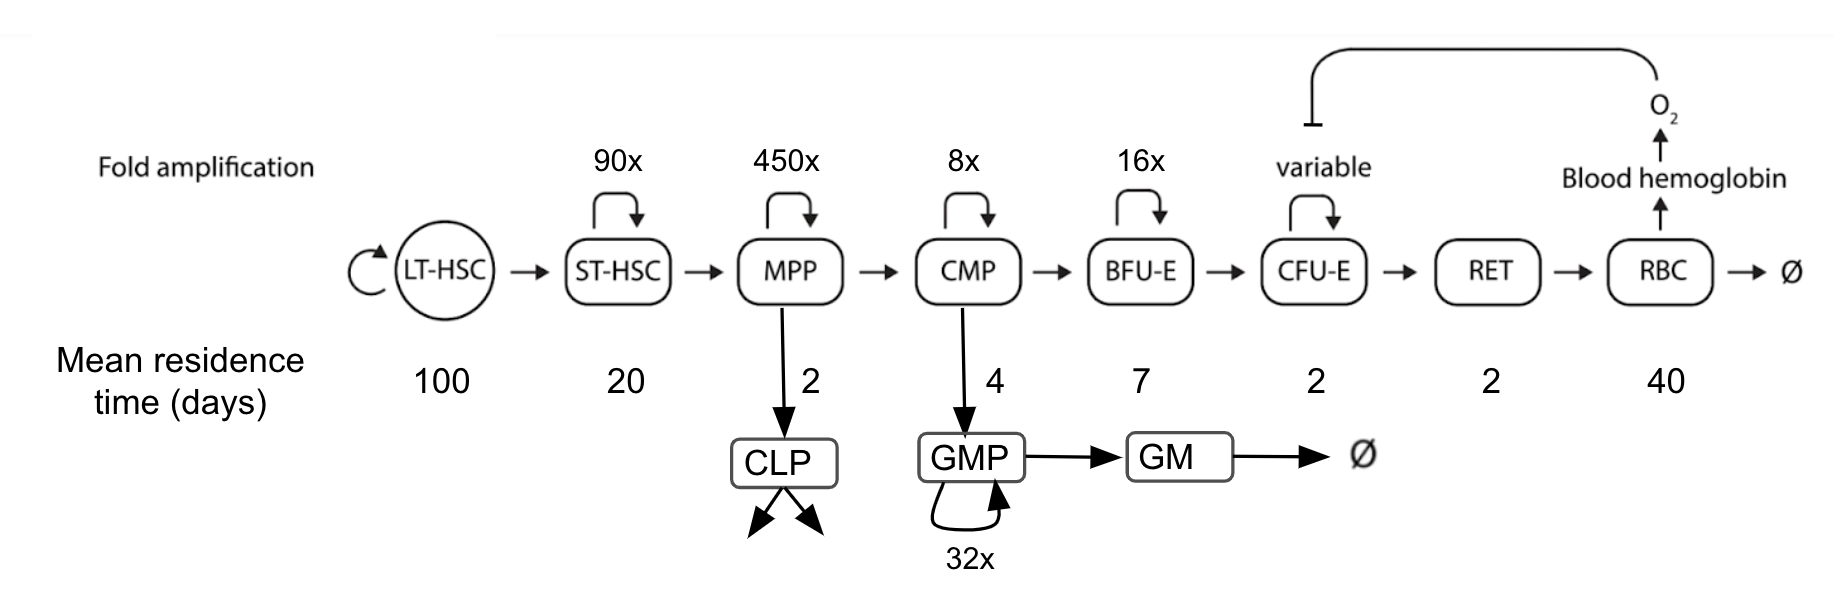
\includegraphics[width=\textwidth]{../img/mouse_full_model.png}
\end{minipage}
\hspace{0.5cm}
\begin{minipage}[b]{0.4\linewidth}
\centering
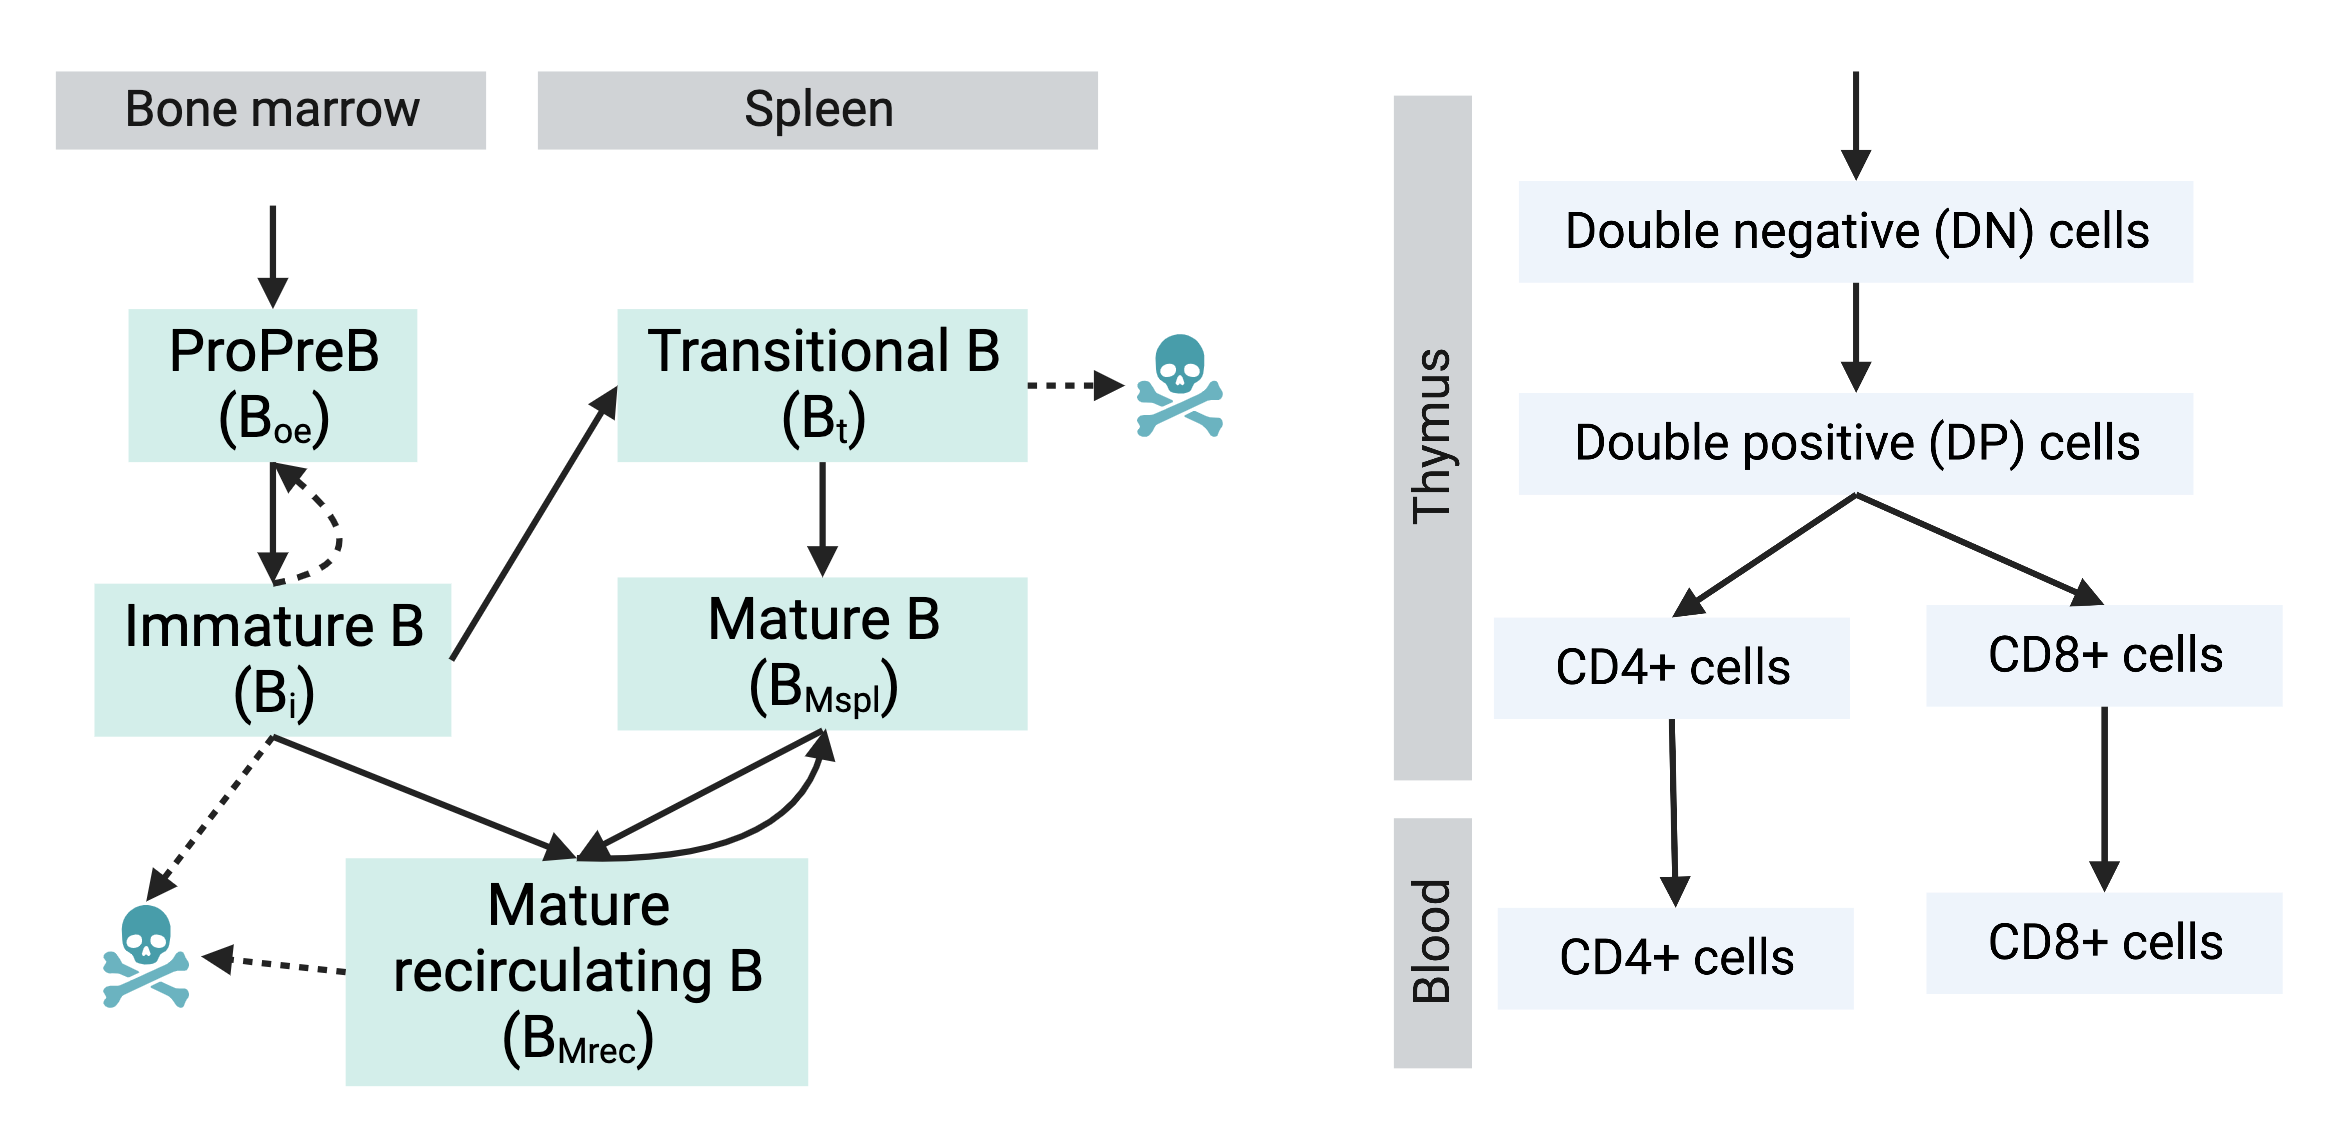
\includegraphics[width=\textwidth]{../img/Diagram_B_T.png}
\end{minipage}

The steady state of this model simulation compared well with mouse physiological data reported in literature. 
Furthermore, we demonstrate the model can predict the reconsititution dynamics of RBC, B cells, and T cells after HSC transplant in mouse published in Busch et al., Nature. 2015.  

\begin{minipage}[ht]{0.42\linewidth}
\begin{center}
\fontsize{6.5pt}{6.5pt}\selectfont
\begin{tabular}{ c c c }
Cell type & Simulated & Reference \\ 
\hline
\scriptsize
MPP & 60k & 75k-92k \\  
CMP & 2M & 755k- 3M  \\
GMP & 757k & 1M  \\  
GM & 8.4k/uL & 1.95-12.01k/uL \\  
RET & 498k/uL & 200 - 500k/uL   \\    
RBC & 9.9M/uL & 10.2M/uL   \\ 
blood Hb & 13.2g/dL & 13.6 - 16.4g/dL   \\ 
Hb in RBC & 261g/L & 270-330g/L  \\ 
lymphocyte & 1.8k/uL & 0.12 - 24k/uL  \\ 
\hline
\end{tabular}
\end{center}
\end{minipage}
\hspace{0.2cm}
\begin{minipage}[ht]{0.5\linewidth}
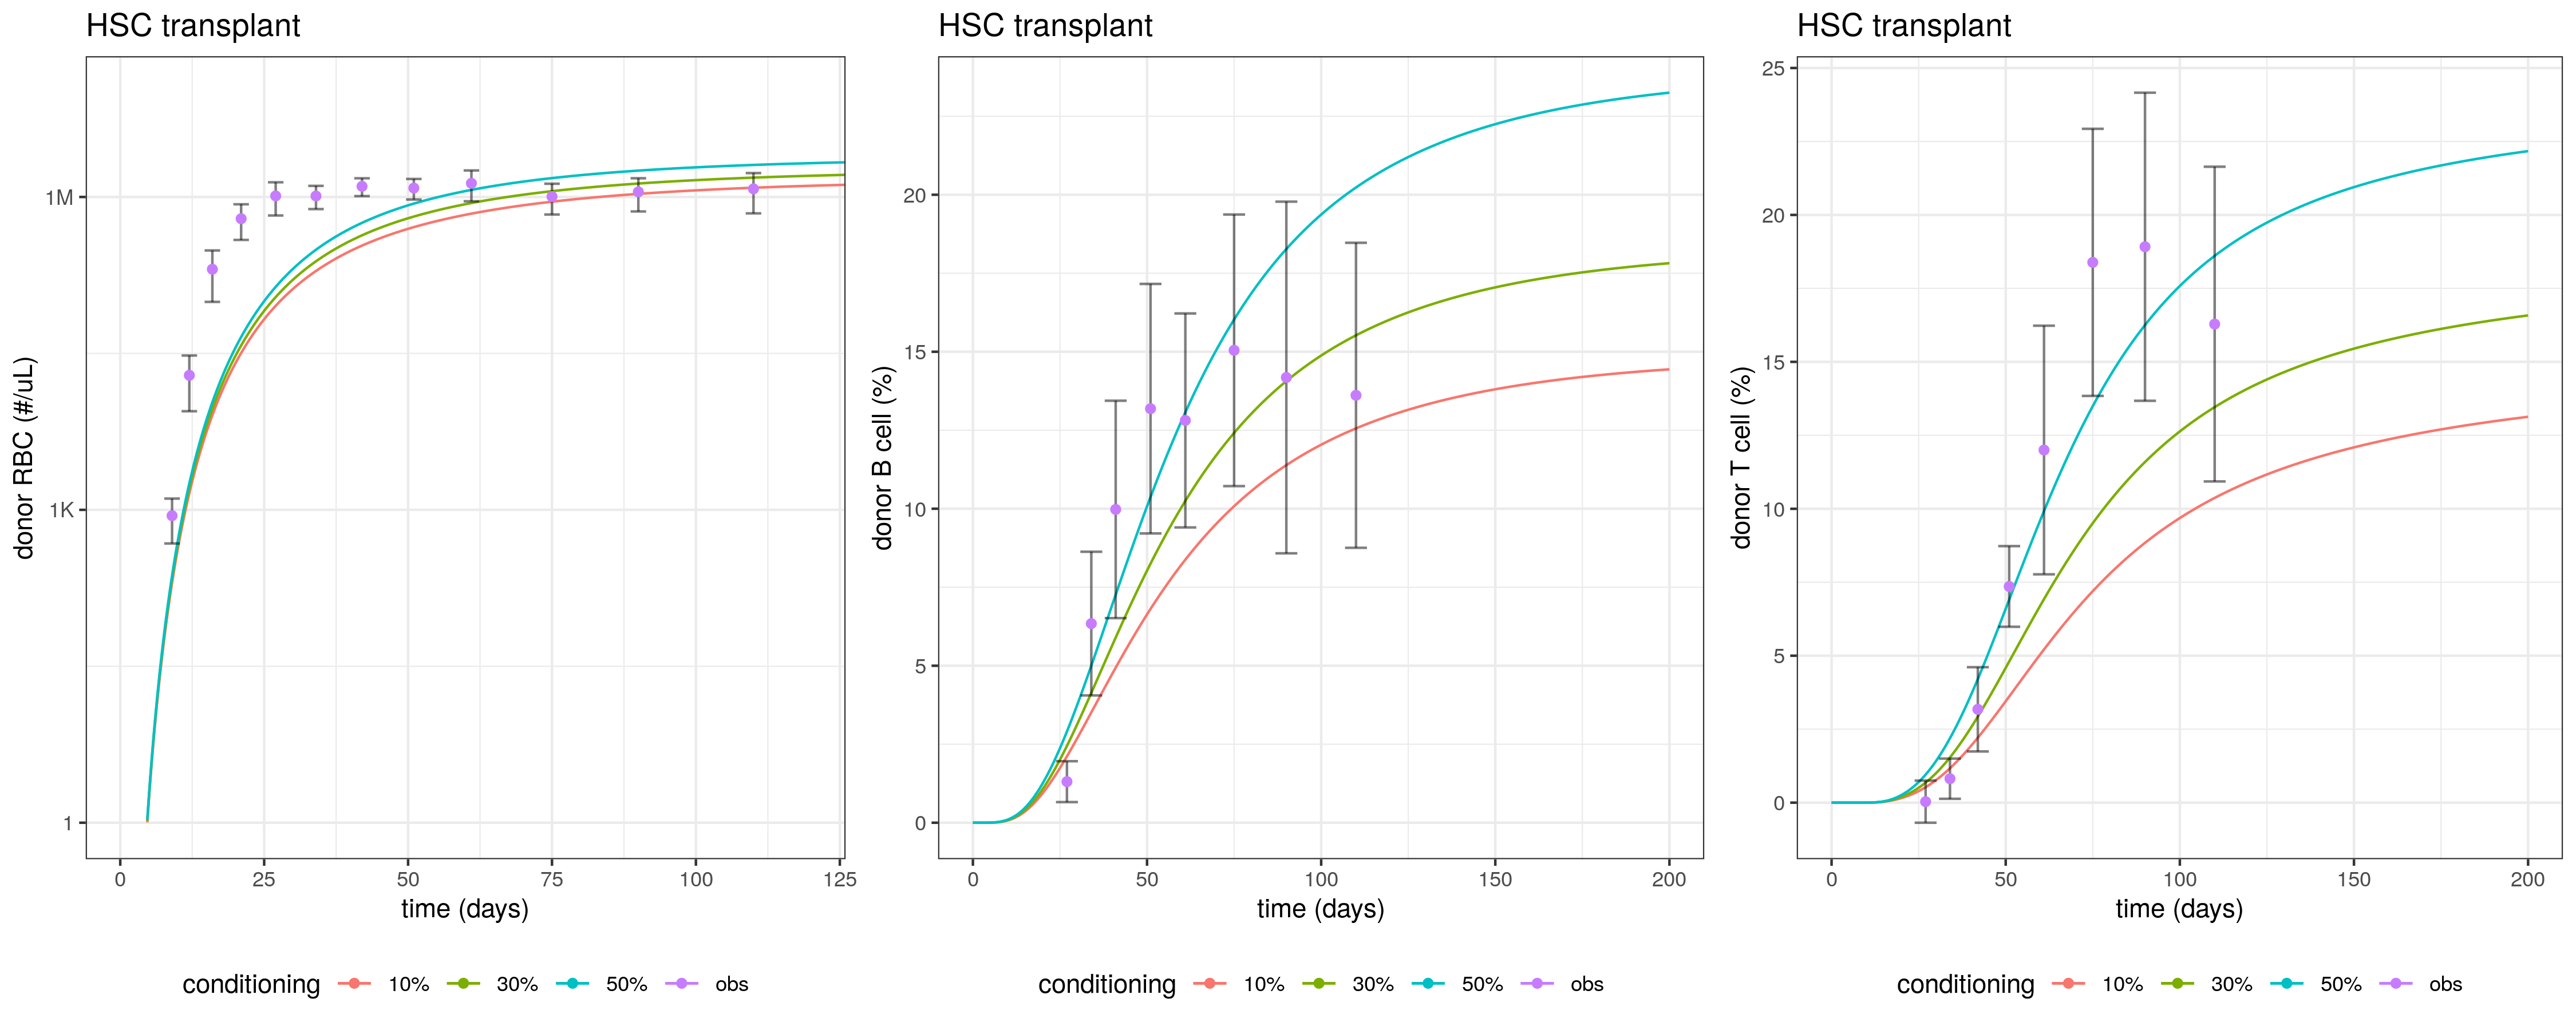
\includegraphics[width=\textwidth]{../img/mouse_RBC_T_B_HSCT.png}
\end{minipage}

The integrated HSC differentiation model for human can be summarized by the figure follow. Briefly, the model was scaled from mouse to human. Especially, the scaling of bone marrow B cell capacity was scaled based on cellularity. In addition,naive T cell dynamics in lymph nodes (LN) and peripheral tissues from [4] was also incorporated to capture the different mechanism in T cell maintenance: in mouse, thymic output is the main source of naive T cell maintenance; in human, naive T cell proliferation in peripheral tissue and blood have a prominant role (Famili et al., Future Sci OA., 2017, Spits, Curr Opin Immunol., 1994). 

\begin{minipage}[b]{0.55\linewidth}
\centering
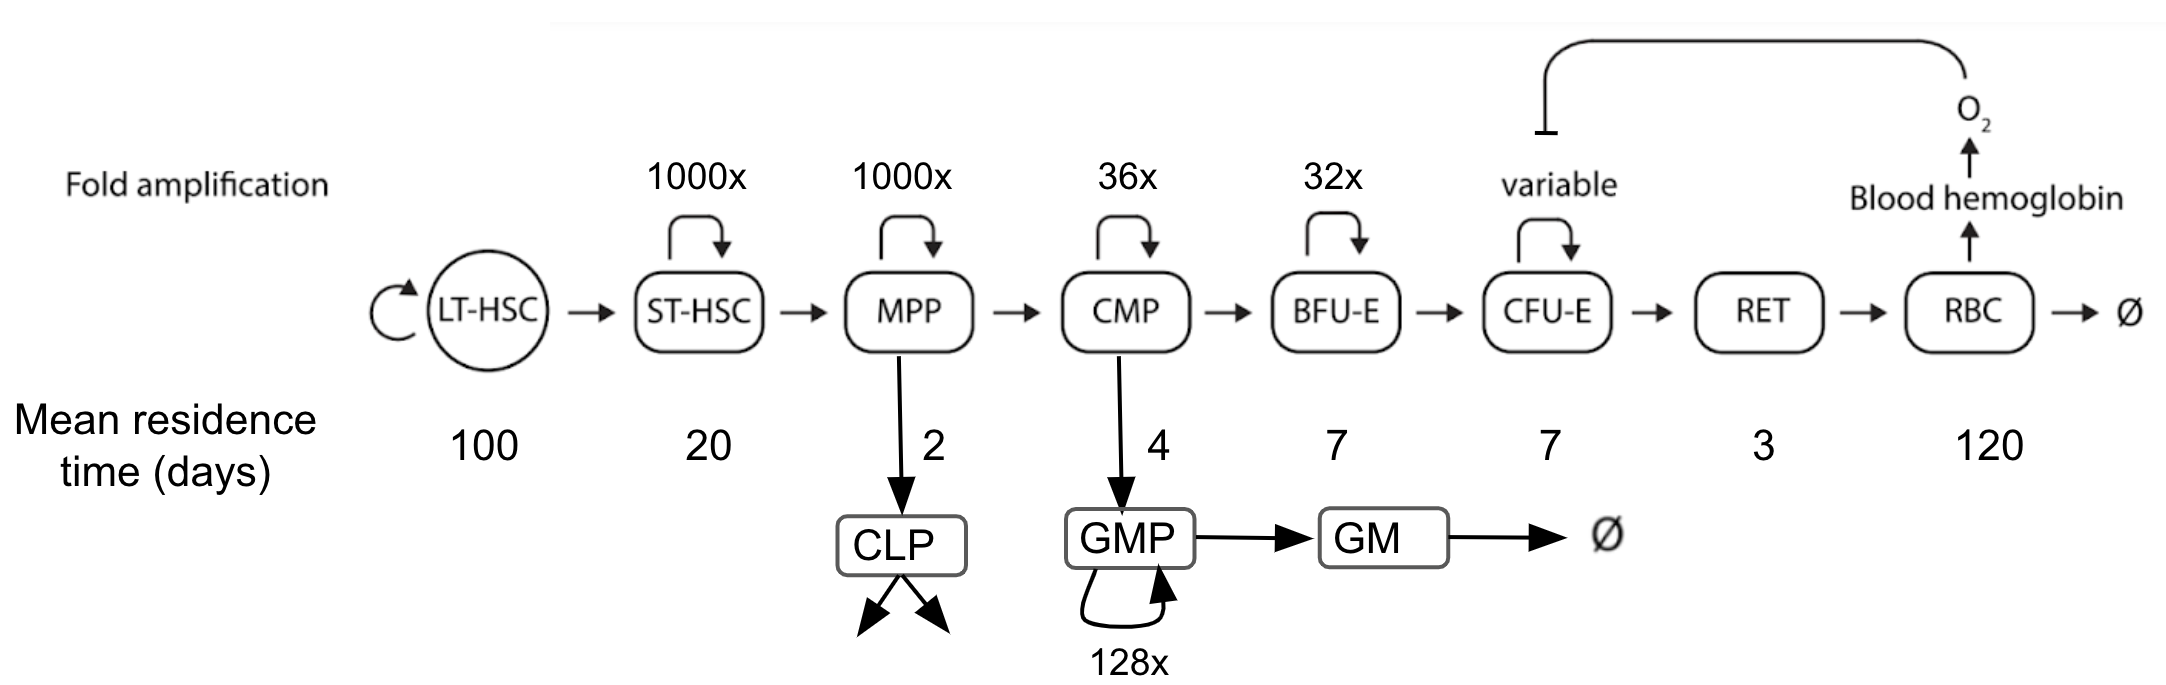
\includegraphics[width=\textwidth]{../img/human_full_structure.png}
\end{minipage}
\hspace{0.5cm}
\begin{minipage}[b]{0.4\linewidth}
\centering
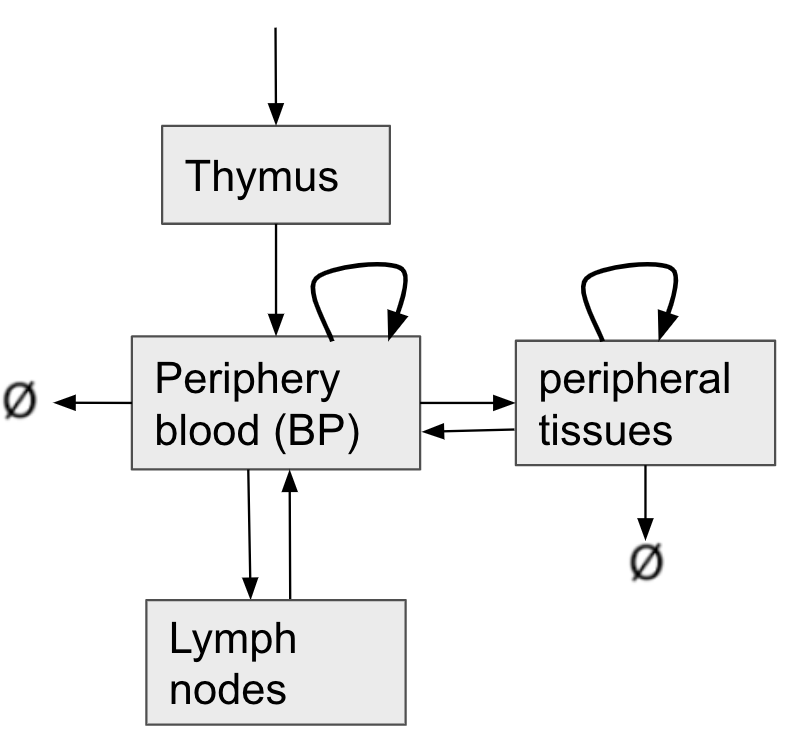
\includegraphics[width=\textwidth]{../img/human_naiveT.png}
\end{minipage}


The model was firstly used to simulate steady state blood cell, hemoglobin, and immune cell in both healthy situation and patients with adenosine deaminase deficiency severe combined immunodeficiency (ADA-SCID). Note for those with ADA-SCID, the death rate of DP cells in thymus and splenic mature B cells were adjusted based on data obtained from mouse (Whitmore and Gasper et al., Front Immunol., 2016, Blackburn and Kellems et al., J Exp Med., 2000, Moretti et al., Sci Rep., 2021). 

\begin{minipage}[ht]{0.4\linewidth}
\begin{center}
\fontsize{6.5pt}{6.5pt}\selectfont
\begin{tabular}{ c c c }
Cell type & Simulated & Reference \\ 
\hline
\scriptsize
RBC (/uL) & 3.9M & 4M \\  
Hb (g/dL) & 13.2 & 12-15  \\
thymic output (/day) & 32M & 10M-2700M \\  
granulocyte (/uL) & 1.2k & 1k-8k   \\ 
T cell (heathy) (/ul) & 662 & 1243   \\ 
T cell (ADA-SCID) (/ul) & 149 & 138  \\ 
B cell (healthy) (/uL) & 137 & 101 \\
B cell (ADA-SCID) (/uL) & 61 & 0  \\
\hline
\end{tabular}
\end{center}
\end{minipage}
\hspace{0.2cm}
\begin{minipage}[ht]{0.3\linewidth}
\end{minipage}


The model was used to simulate blood cell and hemoglobin reconstitution after a patient treated for sickle cell disease (SCD), as well as immune cell reconstitution for a patient treated for ADA-SCID. 

The simulated result of SCD treatment was compared to data published in Ribiel et al., N Engl J Med., 2017 (left panel). The model captured the lowering of RET count up to 6 months after the gene therapy, as well as the increase of HbA$^{T87Q}$, a Hb that only exists in transduced cells. The mismatch in HbA and RBC count at 3 months after the gene therapy could be due to the transfusion received by the patient. 


The simulated result of ADA-SCID patient was compared to a patient reported in Aiuti et al., N Engl J Med., 2009 (right panel). Note the total amount of CD34+ cells infused into this patient was estimated based on the patient's age and gender (seven-month old female). The simulated result on B cell and T cell reconstitution matched up well with observed data. The simulation on granulocytes matched less well in the later years. It may suggest the myeloid arm of this model could be further refined. 

\begin{minipage}[b]{0.47\linewidth}
\centering
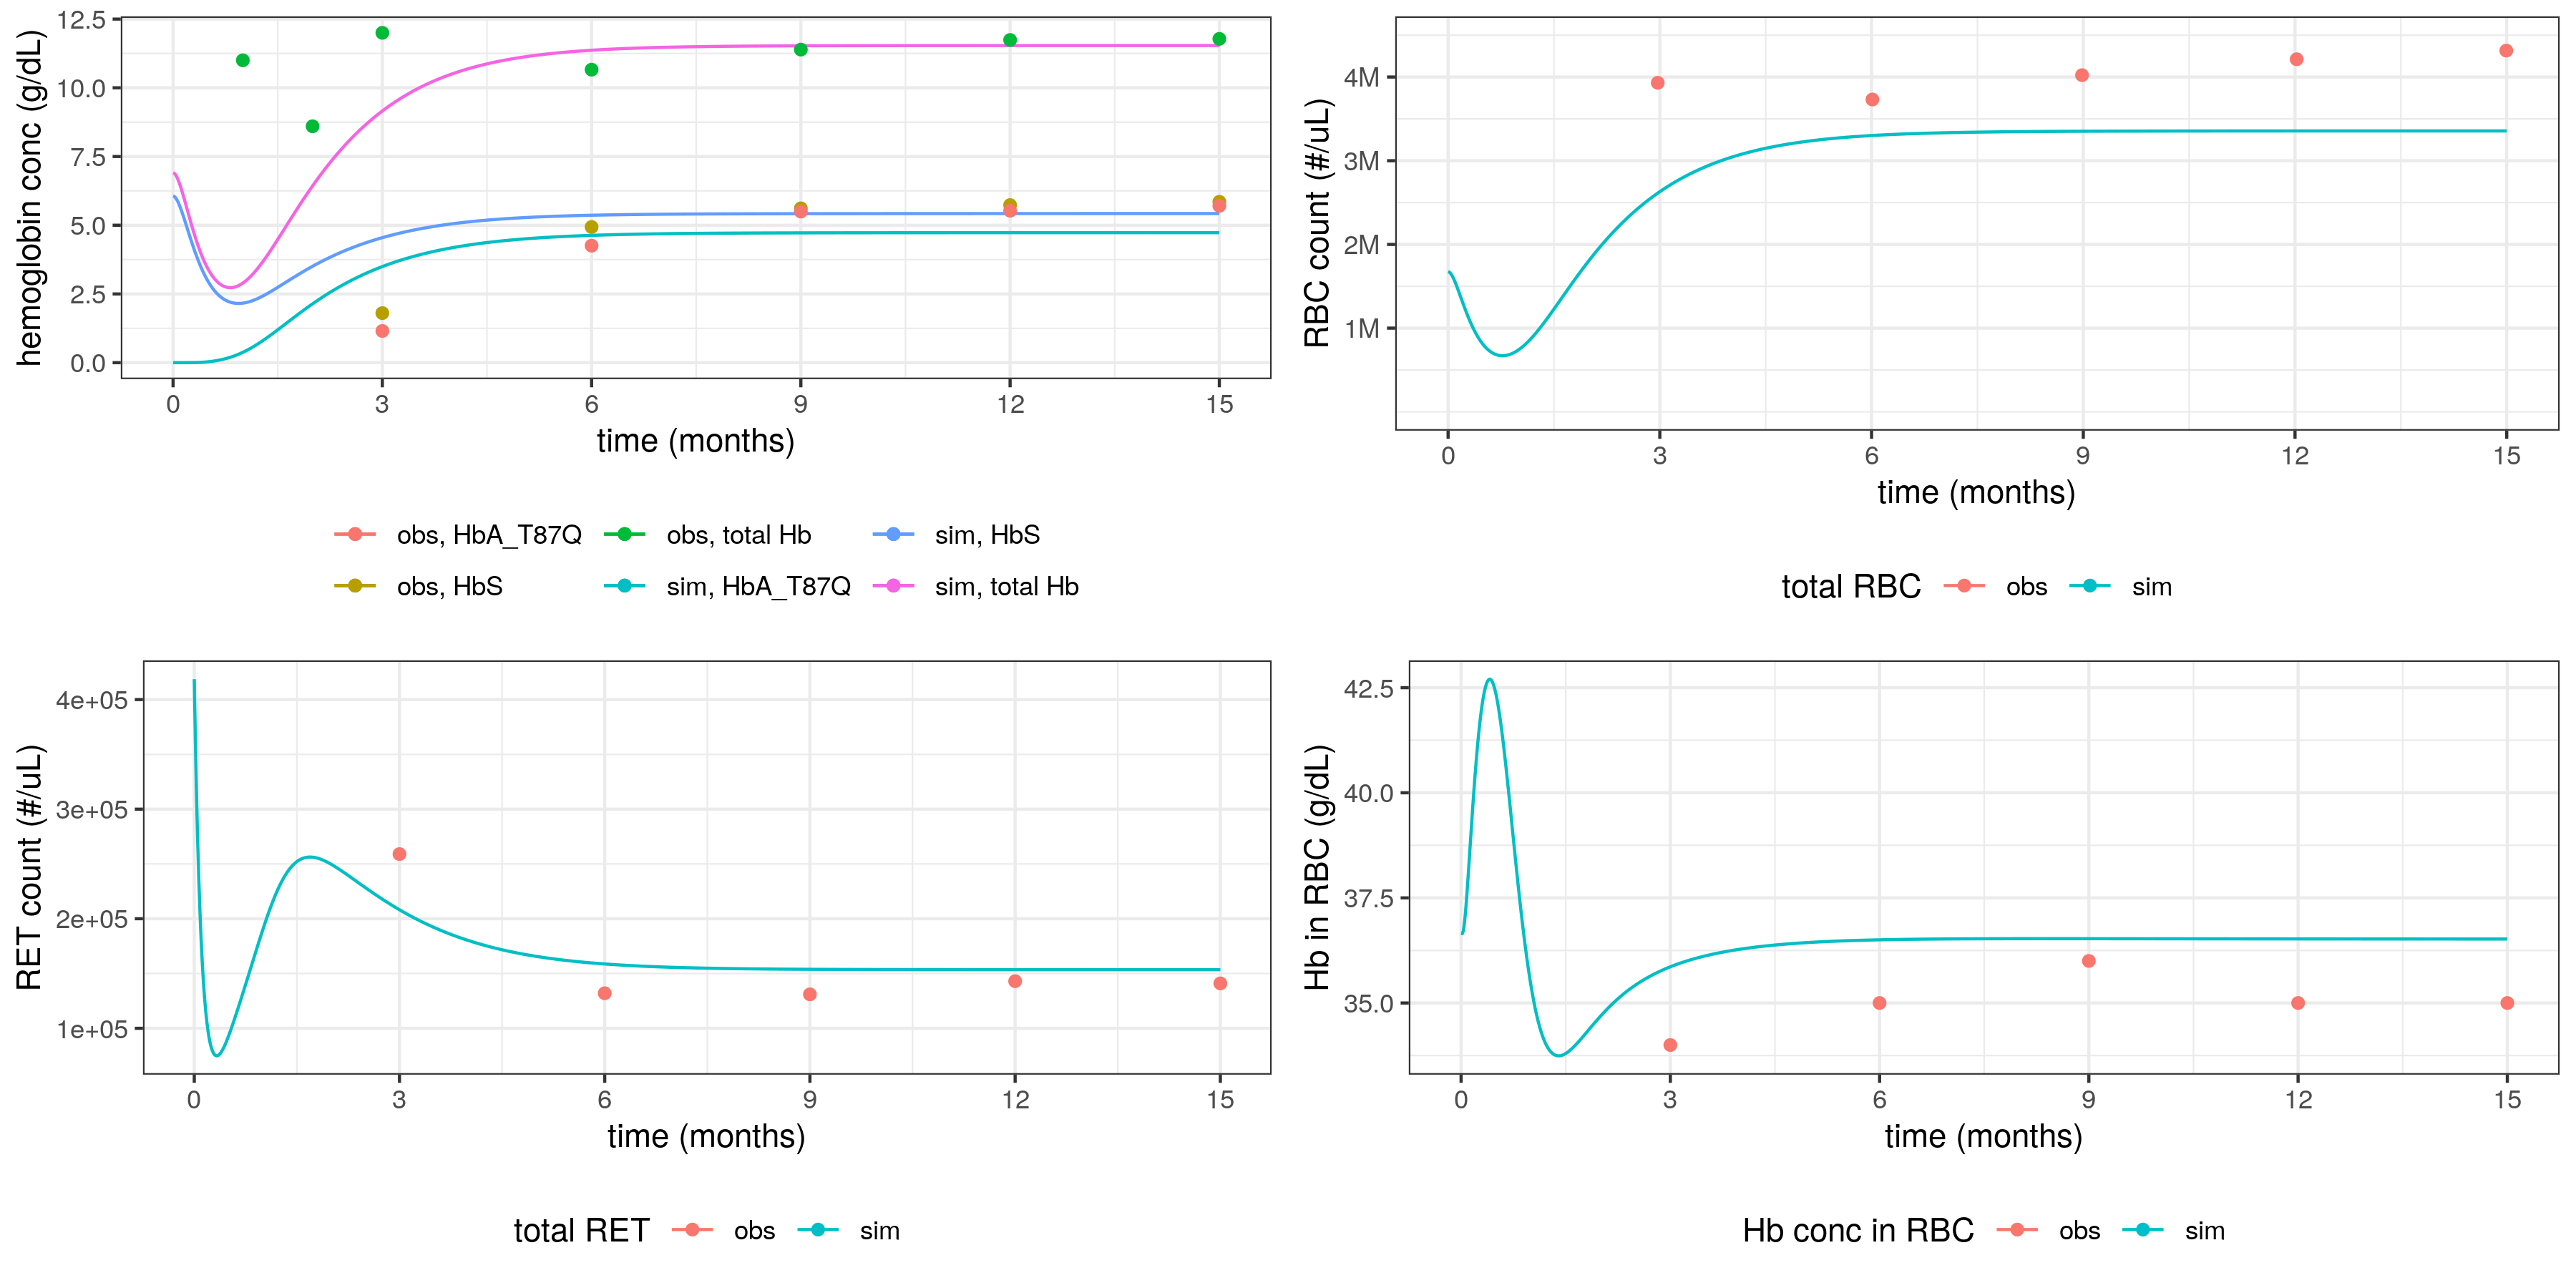
\includegraphics[width=\textwidth]{../img/human_erythroid_validation.png}
\end{minipage}
\hspace{0.5cm}
\begin{minipage}[b]{0.47\linewidth}
\centering
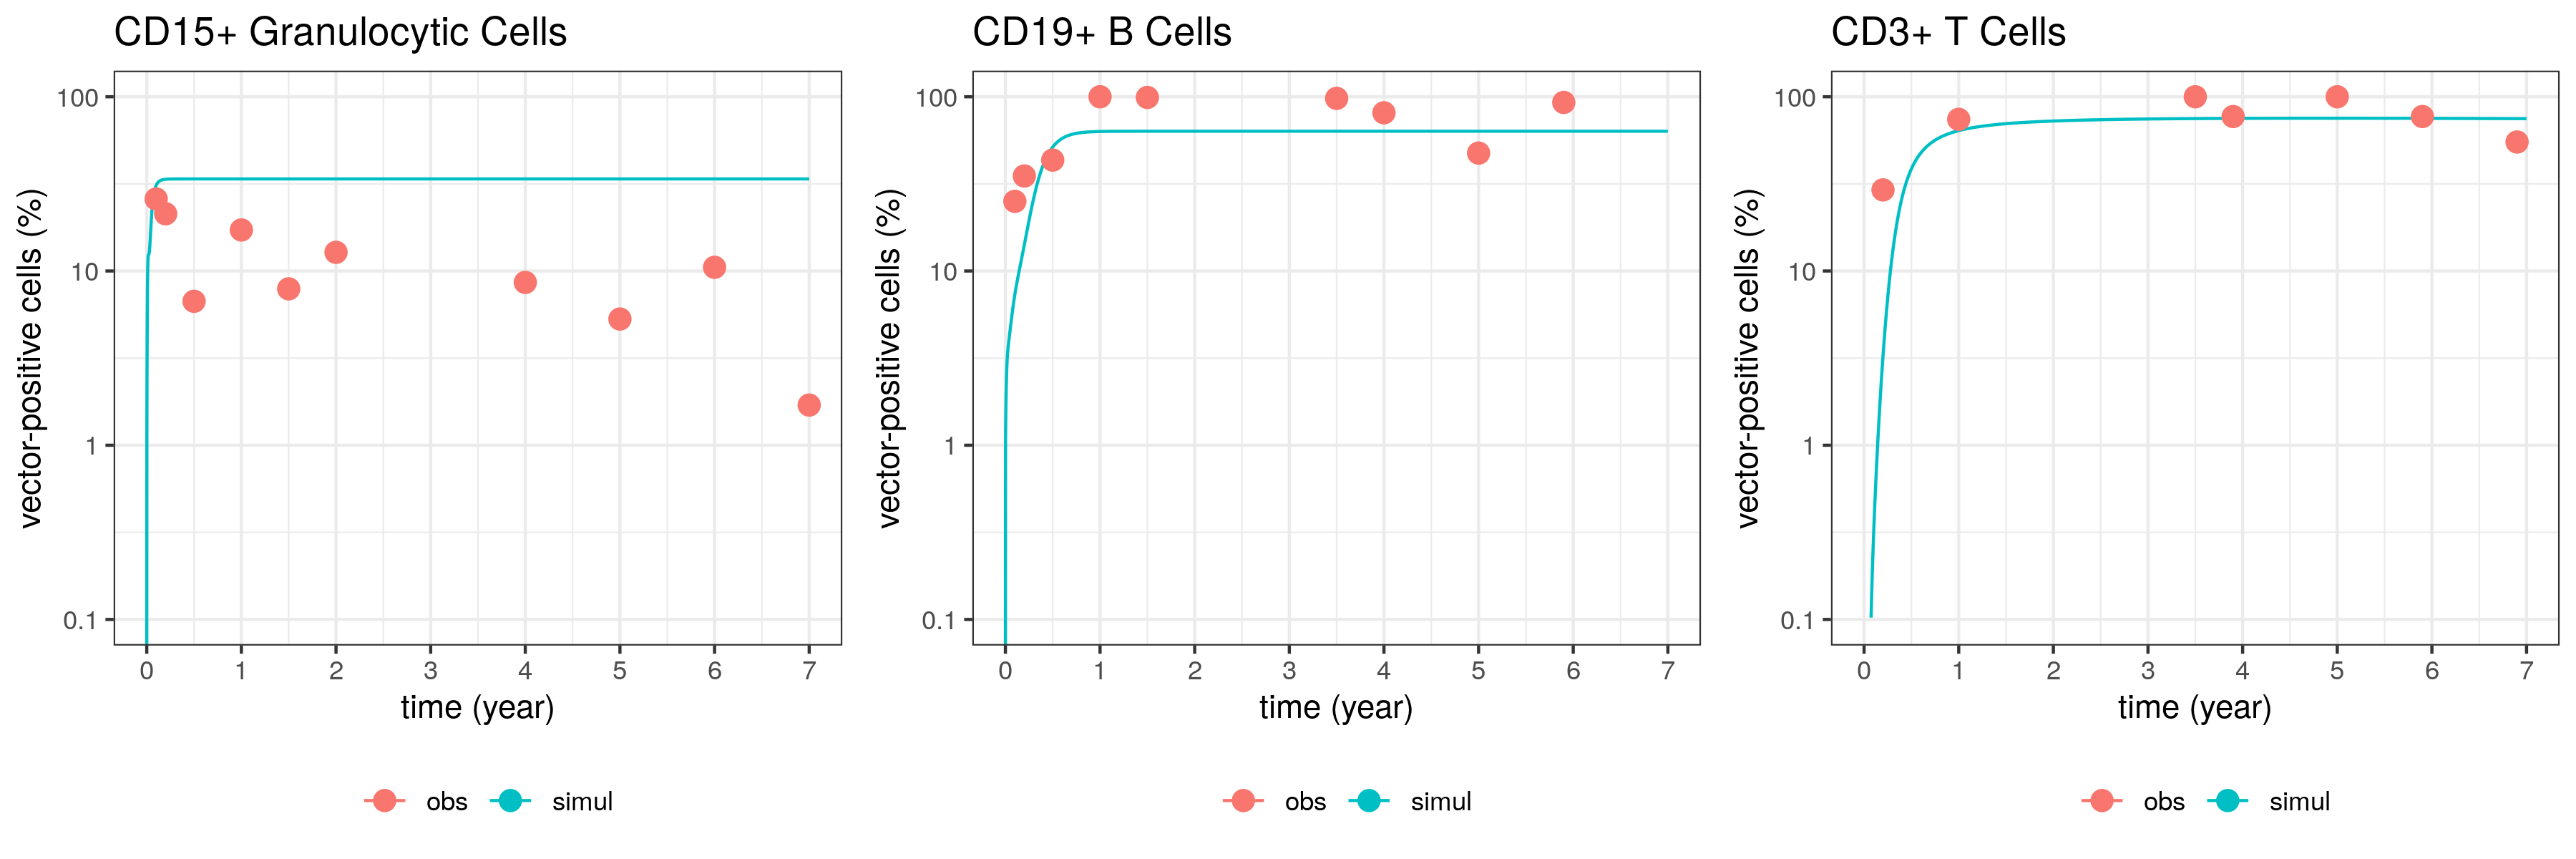
\includegraphics[width=\textwidth]{../img/human_ada_scid_GT.png}
\end{minipage}





}

%%%%%%%%%%%%%%%%%%%%%%%%%%%%%%%%%%%%%%%%%%%%%%%%%%%%%%%%%%%%%%%%%%%%%%%%%%%%%%%%


\headerbox{Conclusion}{name=conclusion,span=2,column=1,below=results}{
\footnotesize
Our work has resulted in a more comprehensive representation of mammalian hematopoietic stem cell development than previous partial efforts. Our integrated model is based on physiological understanding and validated with both mouse and human data. The models are implemented in both R and Julia, and the code will be available on GitHub. We believe this integrated model provides a versatile platform for predicting cell reconstitution after HSC transplant or ex-vivo gene therapy. 
}

\end{poster}
\end{document}
